% !Mode:: "TeX:UTF-8"

\documentclass[11pt, a4paper]{article}
\usepackage{xltxtra,fontspec,xunicode}
\usepackage{amsmath}
\usepackage{amssymb}
\usepackage{amsfonts}
\usepackage[slantfont,boldfont]{xeCJK} % 允许斜体和粗体

\usepackage{indentfirst}
\usepackage{caption}

\setCJKmainfont{STSong}
\setCJKmonofont{SimSun}
\usepackage{geometry}
\usepackage{graphicx}

\geometry{top=1in, bottom=1in, left=1in, right=1in}
\linespread{1.5}

\DeclareMathOperator*{\argmax}{argmax}
\DeclareMathOperator*{\argmin}{argmin}

\newcommand{\degc}{$\,^\circ$C}


\begin{document}



\title{Title}
\author{滕达\footnote{北京大学化学与分子工程学院、定量生物学中心,通讯地址:\texttt{tengda@pku.edu.cn},$\mathrm{id}=1500011735$},乔卓然\footnote{北京大学化学与分子工程学院、生物动态光学成像中心,通讯地址:\texttt{utenaq@pku.edu.cn},$\mathrm{id}=1500011826$}}
\date{\today}

\maketitle

在生物物理领域,荧光共振能量转移(FRET)是一种根据荧光信号随时间的涨落探测蛋白质、核酸等生物大分子动力学信息及其结构性质的有力手段;分子中的荧光基团之间的距离与荧光发射的效率成负相关,采集到的荧光信号发射效率也称为该分子的FRET效率。荧光效率的高低对应着分子内两个荧光基团之间的瞬时距离,这使得分子在微观层次成为一个精巧的“荧光开关”,伴随着这个分子开关在不同微观状态之间发生翻转,荧光同步地发生亮/暗变化,而实验上会观测到荧光强度(FRET 效率)随时间的高低跳跃轨迹。随着技术的发展,实验中可以获取单个生物分子的荧光信号轨迹,从而推断单个分子在微观层面的结构与动力学性质,这一方法称为单分子FRET技术。
\begin{figure}[htb]
  \centering
  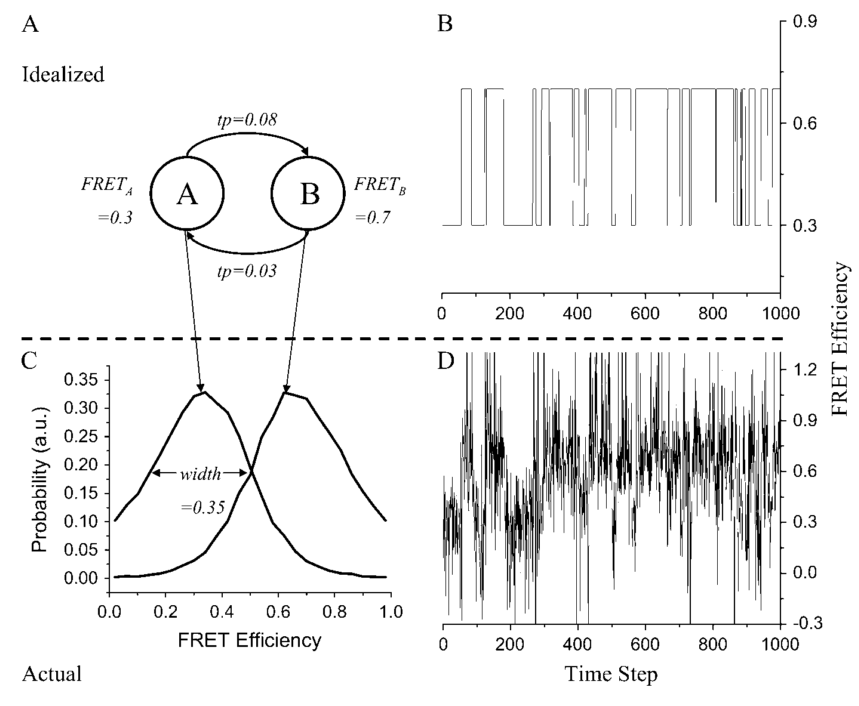
\includegraphics[height=11cm]{Fig_trace.PNG}\\
  \caption{对存在两个微观状态的分子进行荧光观测,上图为理想情形下状态转移模型和对应的FRET 轨迹, 下图为实际FRET发射效率的概率分布和一条实际获得的FRET 荧光轨迹.}
  \label{fig:trace}
\end{figure}

在理想情形下,目标分子的微观状态是离散化的,且单个状态只对应一个特定的FRET荧光效率(Figure \ref{fig:trace}a);随着分子在不同状态之间的转变,收集到的信号应当为不同荧光效率大小的时间序列,形似方波,不同微观状态可以直接通过荧光效率的高低辨别得到(Figure \ref{fig:trace}b)。但在实际实验中,构象和荧光强度的涨落使得收集到的荧光轨迹呈现为高度随机化的轨迹(Figure \ref{fig:trace}c, d).因此,如何通过有效的数学建模,发展由随机化的单分子FRET 荧光轨迹解析出不同微观状态和状态间转移事件的方法则成为研究者尤为关注的课题。


\section{Simple HMM}\label{chapter:HMM}
\subsection{荧光轨迹分析问题}

2006 年Sean A. Mckinney 等人首先建立了应用基于最大似然估计(Maximum Likelihood Estimate, MLE)的隐式马尔科夫模型分析单分子FRET荧光轨迹的方法\cite{HMM};由于实验中物理测量的信号强度都是测量时间内的平均值,是一个间接观测量;而实际的分子微观状态则是对应的隐过程,荧光信号序列分析的建模需求与HMM 模型的思想不谋而合。

在Mckinney 等提出的HMM 模型中,FRET荧光轨迹作为观测量的离散时间序列$y_i$,对应着在$i$ 个时间步长后$t=\{\delta t,2\delta t,3\delta t…\}$ 观测到的荧光效率;分子的微观状态设为离散的隐变量$z_i$,构成状态链$z=\{z_1,z_2,...,z_N\}$;不同微观状态之间在一个时间步长后发生转变的概率通过概率转移矩阵$a_{z_{i}, z_{i+1}}$ 给出;而分子处于某一微观状态时观测到的FRET 效率的概率分布可以通过连续的观测概率条件分布函数给出,且近似服从高斯分布(Figure \ref{fig:trace}c):
\begin{equation}
p(y|z) \propto \exp\left[-2\times\left(\frac{y- y_z}{\sigma}\right)^2\right]
\end{equation}
其中$y=\{y_1, y_2,\cdots, y_N\}$为观测到的FRET效率序列,$y_{z}$ 为理想情形下微观状态$z$ 对应的FRET 效率大小。

对于该HMM模型,需要确定三部分未知参数:分子的总微观状态数$S$,微观状态之间的状态转移矩阵$a_{z_i, z_{i+1}}$以及各个状态的发射概率分布的均值$y_{z}$及峰宽$\sigma$。 如果给定总微观状态数$S$,模型参数的估计可以采用ML法处理,通过遍历由$a_{z_{i}, z_{i+1}}$, $y_{z} $和$\sigma$组成的状态空间优化荧光轨迹的总观测概率$p(y| \lambda)$得到。FRET 的总观测概率$p(y|z,\lambda)$ 由下式给出。我们可以根据这个概率对$z$和$\lambda$ 分别做优化。
\begin{equation}
p(y|z,\lambda)= \prod_i^N p(y|z) a_{z_{i}, z_{i+1}}
\end{equation}


对于$z$的优化,计算过程中需要先对每组$\lambda$ 的猜测值做优化,即
\begin{equation}\label{eqn:z_opt}
  z^*=\argmax_z p(y|z, \lambda)
\end{equation}
如果直接遍历隐状态链$z$,这一过程的计算复杂度将达到无法承受的$O(S^N)$。幸运的是,通常的荧光实验要求分子性质保持稳定,因此可以假设$a_{z_{i}, z_{i+1}}$与$i$ 无关;引入这一假设后问题被大大简化,通过应用Viterbi算法即可将计算复杂度降到$O(N)$ 量级。
\begin{equation}
\lambda^*=\argmax_{\lambda} P(y|z,\lambda)
\end{equation}

确定了由一组给定$\lambda$ 求解最优的$z*$ 和相应的$p(y|z,\lambda)$ 的方法,就可以通过优化后验概率$p(y|z^*,\lambda)$ 求得$\lambda^*$。 这个选择模型参数的过程可以由常规的多维优化算法完成,例如Mckinney 采用了Brent–Dekker算法解决了这一问题\cite{Brent}。参数$\lambda$的初始猜测则可以由一个时间步长内的$y\rightarrow y'$ FRET转移概率密度图近似给出(Figure \ref{fig:tdp}),转移密度函数$p(y,y')$定义为:
\begin{equation}
p(y,y')=\sum_{z=1}^S \sum_{z'=1}^S A_{z, z'} \exp\left[-\frac{(y- y_{z})^2+(y'- y_{z'})^2}{\sigma^2}\right]
\end{equation}

其中$A_{z,z'}$是一个步长后隐状态由$z$跳至$z'$事件的总计数。转移概率密度p(y,y')可以直观地反映对于任意的微观状态转换事件,发生状态转换的一个步长前后FRET效率由$y$ 跳至$y'$ 的概率。转移概率密度图的峰值意味着有高概率发生$y\rightarrow y'$的转换,我们可以将峰对应的$y$作为$y_z$的初始值,归一化后的峰高积分对应$a_{z_{i}, z_{i+1}}$的初始取值。

\begin{figure}[htb]
  \centering
  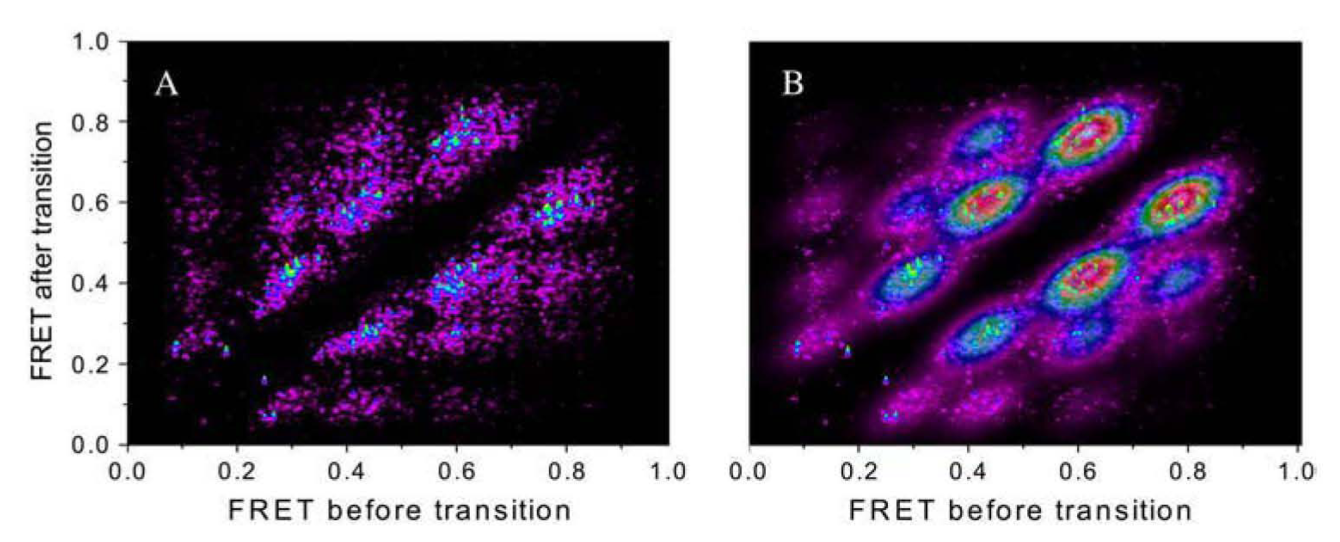
\includegraphics[height=6.5cm]{Fig_tdp.PNG}\\
  \caption{对于一个含有5 个状态的模型生成的荧光轨迹,A为用初始值(其中$\sigma^2=0.0005$,表现为样点离散分布)计算得到的FRET转移概率密度图,B 为进行参数优化后的转移概率密度图,可以从中指认集中出现的微观状态和状态转换事件。}
  \label{fig:tdp}
\end{figure}

%如果对于不同分子测定了多条荧光轨迹,为了提高参数的预测精度,模型参数的优化...

对于微观状态数$S$ 的估计,一个直接而简便的方法是首先假定存在大量的微观状态,之后直接通过HMM进行拟合,在模型收敛后,舍去对转移概率矩阵的贡献小的状态,可以忽略或人为舍去。很显然直接进行多状态拟合的准确度强烈依赖于荧光数据质量。为了获得更为可靠的预测结果,还可以采取遍历不同S值估计最优状态数的策略,例如使用贝叶斯信息准则(Bayesian Information Criterion)来评估分子状态数为S 的可能性:
\begin{equation}
BIC(S)=-2ln[p(y,z|\lambda)]+(S^2+1)ln[p(z|\lambda)]
\end{equation}


此时对S的优化转化为求BIC 的极大值,这一过程同样也可通过Brent–Dekker 算法进行。Mckinney等还通过模拟数据和核酸分子折叠的单分子FRET实验数据对模型进行了测试(Figure \ref{fig:test}),在不同状态之间荧光效率均值相差0.1 以上,观测函数峰宽小于0.4 时表现较好。

\begin{figure}[htb]
  \centering
  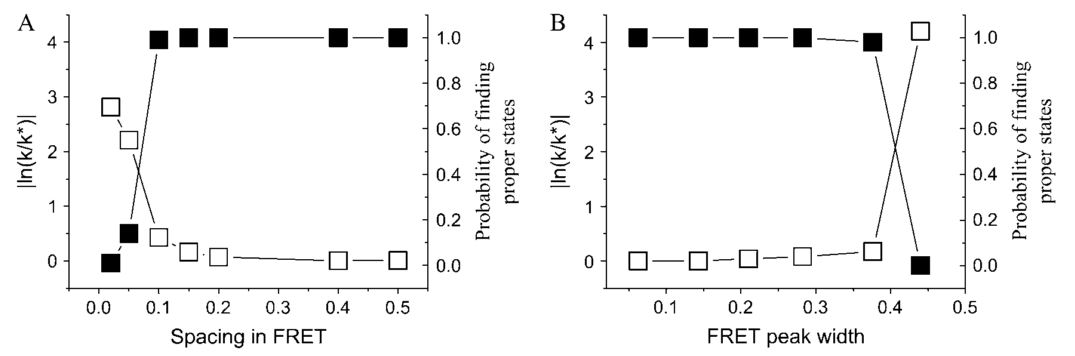
\includegraphics[height=5cm]{Fig_test.PNG}\\
  \caption{通过包含2个微观状态,设置不同参数生成的模拟轨迹测试HMM模型表现。每条轨迹步数为1000,左右纵坐标分别为状态转移概率预测值$k$ 和实际值$k^*$的平均对数差以及预测得到正确状态数S的频率。分别统计不同参数变化对模型表现的影响:(A) 两态荧光效率差异, (B) FRET效率分布峰宽。}% (C)微观状态寿命, (D) 状态转换事件数。
  \label{fig:test}
\end{figure}

然而该模型的一个不足之处在于,如果直接假定较大的状态数S进行拟合将易于发生过拟合现象,模型可能将噪声涨落带来的高低荧光信号识别为不同微观状态,得到没有实际意义的多状态数预测结果。使用BIC 判据进行S 的选择将问题转变为寻找最可靠的总微观态数,这可以改善过拟合带来的问题;然而遍历S的过程其实隐含地假设了S的先验概率相等,这意味着这一基于ML算法的模型并未真正判断是否发生了过拟合,仍然会接受S数目很大时的参数估计。这同时也降低了对噪声的抵抗能力,$\sigma$较大时模型表现较差,而$\sigma$在实际荧光实验中会随着时间步长$\delta t$ 的减小而上升,Mckinney 等提出的HMM算法距离高时间分辨率下广泛的实验应用仍有一定距离。此外,通过优化$\lambda$使得要获得较高的精度必须尽可能缩短差分步长,这一经典HMM 方法需要循环迭代$S$,$\lambda$和$z$,随着体系复杂度的上升计算开销也将显著增大。


\subsection{HMM方法的扩展}
\textcolor[rgb]{1.00,0.00,0.00}{\texttt{Move this subsection}}

除了常规的HMM模型,我们在接下来的章节会介绍一些改进的HMM模型,它们改进了实验的分辨率或从荧光轨迹中挖掘出了更多的信息。

第\ref{chapter:H2MM} 章中,我们介绍了一个提高分辨率的实验手段。常规的实验测量中,每一个测量点对应的都是大量光子被探测到之后均值化之后的结果。为了获得更短时间尺度的更细节的状态转移信息,我们需要进行单光子的测量。但单光子发射事件之间可能发生多次的状态转移,时间尺度出了问题。为了直接将单光子发射和状态转移关联起来,我们需要一些额外的数学手段。

而在Mckinney的工作中,简单HMM对于噪声有比较强的敏感性。估计微观状态数$S$成了一个难题。我们在第\ref{chapter:VBEM} 章讨论了一种可以更好的平衡拟合表现和过拟合之间的方法。


\section{H$^2$MM Model}\label{chapter:H2MM}

    为了获取更高的时间分辨率来解析更精细的蛋白质动力学,Menahem Pirchi等人建立了单光子观测的实验手段\cite{H2MM}。 由于在实际的蛋白质荧光光谱中,两次接收到光子的时间不可能无限的短。因而,当我们把时间步长$\delta t$ 取得足够小的时候,在一个$\delta t$ 内系统收到两个光子的概率事实上可以忽略不计。因此,在实际使用的$\delta t = 1\,$ns 的时间步长下,这个问题已经可以看成离散时间的马尔可夫模型。

    但这个问题和序言中所提到的简单隐马尔可夫模型有显著区别。在传统的荧光观测中,观测的步长足够长,因此每个步长内都可以测量出一个荧光强度(或荧光效率)。而为了获得更短时间尺度下更细节的动力学信息,需要从系统发射的单个光子中解析信息。此时,HMM 使用的时间步长$\delta t$ 很短,在两次发射光子时间之内可能系统已经发生了若干次状态转换。因此,光子到达的时间序列并不能完整地包含关于体系状态改变的信息。由于额外的这层信息丢失,我们必须在系统的状态转移和光子测量的时间序列之外再增加一个参量来将他们联系起来。因此,这个模型被称之为H$^2$MM.

    我们假设两次收到光子之间的时间差$\Delta t_n = t_{n+1}-t_n$, 如果以$\delta t=1\,$ns作为单位,$\Delta t_n$总可以是一个整数。不同于普通的HMM, 在H$^2$MM 中,状态转移矩阵会相应的变成$a_{x_ix_j}^{\Delta t_n}$. 如果将$\Delta t_n$ 固定为1,就可以化为常规的HMM.

    好在,对于已知的实验数据,$\Delta t_n$都是已知的。因此,H$^2$MM仍然可以通过常规的前传算法和后传算法来计算我们感兴趣的$p(x,y|\theta)$. 唯一的区别在于,每次传递的状态转移矩阵$A=a_{ij}$ 需要修改为$A=a^{\Delta t_{ij}}_{x_i, x_j}$.







%% TODO: 统一记号
\section{VBEM Method}\label{chapter:VBEM}

    在实际的荧光轨迹分析中,系统的总状态数在很多情况下是不确定的。因此,马尔可夫模型中的系统的状态数也是不确定的。当选取的模型的复杂度过大,亦即系统的状态数取得过多的时候,就容易出现过拟合。过拟合情况下可以得到极高的后验概率,但却不能从中推断出任何信息。因此,Jonanthan E. Bronson 等人将变分贝叶斯最大期望 (Variational Bayes Expectation Maximization, VBEM) 法应用于隐马尔可夫模型\cite{VBEM},通过给过多的模型参数(即过复杂的模型)以额外惩罚的方式来达到过拟合和拟合不佳之间的平衡。

    \subsection{ML 法与ME 法的比较}
    最大似然估计(Maximum Likelihood, ML)法\cite{wiki:mle} 通过优化一个相似度目标函数$\mathcal L(\theta)$ 来确定模型中的参数$\theta$;而文献\cite{VBEM} 中提出的最可能推断(Maximum Evidence Inference, ME)则可以在不同模型中选择最好的一个。在第\ref{chapter:HMM} 章中提到的ML 方法中,在已知测量值$y$的情况下,可以通过优化$p(y|\theta)$ 来得到最佳的模型参数,即
    \begin{equation}\label{eqn:ML_estimate}
      \theta^* = \argmax_\theta p(y| \theta).
    \end{equation}
    但概率$p(y|\theta)$ 必须是在同一个模型下得到的才有互相比较的意义。因为$p(y|\theta)$ 总是可以通过增加模型的复杂度来变得更大。当离散的实验数据点的个数等于HMM 模型中假设的系统状态数时,$p=1$,达到了绝对的过拟合。因此,仅靠ML 法无法推断关于系统状态数的信息。

    而ME方法则可以用来选择最佳的模型,假设待比较的模型可以用下标$S$来表示,则最佳的$K$ 可以表示为
    \begin{equation}\label{eqn:ME_model}
      S^* = \argmax_S p(y| S) = \argmax_K \int p(y| \theta, S)p(\theta| S)\,\mathrm d\theta
    \end{equation}
    其中,$p(y| S)$中$\theta$ 被积分从而像哑指标一样被消掉(Marginalize),因此也被称之为边际相似性(Marginal Likelihood). 方程中的$p(\theta | S)$ 是各个参数$\theta$ 的先验概率。当模型复杂度$S$ 上升时,$p(\theta | S)$ 会显著下降来拉低$p(y| S)$. 使得过复杂的模型不易出现。Bayes公式将我们感兴趣的$p(\theta|y,S)$ 和边际相似性$p(y|S)$ 和先验概率$p(\theta|S)$ 联系起来。
    \begin{equation}\label{eqn:bayes_vbem}
      p(\theta| y, S) = \frac{p(y| \theta, S)p(\theta| S)}{p(y| S)}.
    \end{equation}
    为了求等号左边的后验概率,等号右边的三个量中我们需要求的只剩$p(y| S)$ 了。其中,$p(y| \theta, S)$是实验测得的。

    从(\ref{eqn:ME_model}) 式中可以看出,$p(y|S)$ 的求解涉及到一个关于$\theta$ 的积分,而$\theta$所构成的空间非常大,这个积分事实上是不可做的。下面我们讨论一种用变分法求$p(y|S)$ 的VBEM 方法。

    \subsection{处理$p(y|S)$的方法}
    上一节的讨论中没有考虑进隐马尔可夫模型中的隐变量$z$,但隐变量不改变整个方法的数学结构,我们可以直接将它加入我们的模型。

    为了简化计算,对于一个后验概率$p(z,\theta|y, S)$,我们可以用类似平均场的方法来构造一个$q(z,\theta)$ 来近似$p(z,\theta|y, S)$. 由$q(z,\theta)$ 的归一性,我们可以写出
    $$\ln p(y|S) = \left[\sum_z\int \mathrm d\theta\, q(z,\theta)\right]\ln p(y|S)$$
    再利用条件概率之间的关系$p(y,\theta,z|S) = p(z,\theta|y, S)p(y|S)$,有
    $$\ln p(y|S) = \left[\sum_z\int \mathrm d\theta\, q(z,\theta)\right]\ln \frac{p(y,z,\theta|S)}{p(z,\theta|y,S)}$$
    在对数的分数线上下同时插入$q(z,\theta)$,并拆开可以得到
    \begin{equation}\label{eqn:supp_21}
      \ln p(y|S) = \sum_z\int \mathrm d\theta\, q(z,\theta)\ln\frac{p(y,\theta,z|S)}{q(z,\theta)}+\sum_z\int \mathrm d\theta\, q(z,\theta)\ln\frac{q(z,\theta)}{p(z,\theta|y,S)}
    \end{equation}
    信息论中著名的Kullback-Leibler 距离给了我们一个估计两个概率分布的接近程度的方法。因此,对于$q(z,\theta)$ 的优化可以写作
    \begin{eqnarray*}
    % \nonumber to remove numbering (before each equation)
      q^*(z,\theta) &=& \argmin_{q(z,\theta)} D_{KL}[q(z,\theta) || p(z,\theta|y,S)] \\
                    &=& \argmin_{q(z,\theta)}\sum_{\{y,S\}} p(z,\theta|y,S)\ln\frac{p(z,\theta|y,S)}{q(z,\theta)}\\
                    &\ge& 0
    \end{eqnarray*}
    等号取到当且仅当$q(z,\theta) = p(z,\theta|y, S)$. 而(\ref{eqn:supp_21}) 式等号右边的第二项就是Kullback-Leibler 距离,而第一项则可以看成是一个$q(z,\theta)$ 的泛函,定义
    \begin{equation}\label{eqn:F_def}
      F[q(z,\theta)] = -\sum_z\int \mathrm d\theta\, q(z,\theta)\ln\frac{p(y,\theta,z|S)}{q(z,\theta)}.
    \end{equation}
    因此,(\ref{eqn:supp_21}) 式可以改写为
    \begin{equation}\label{eqn:supp_24}
      \ln p(y|K)= -F[q(z,\theta)] +D_{KL}[q(z,\theta)||p(z,\theta| y, S)].
    \end{equation}
    有趣的是,如果对$F$进行适当的变形,我们发现$F$ 可以写成类似统计物理中自由能的形式
    $$F[q(z,\theta)] = -\sum_z\int \mathrm d\theta\, q(z,\theta)\ln p(y,\theta,z|K) + \sum_z\int \mathrm d\theta q(z,\theta)\ln q(z,\theta).$$
    如果把$q(z,\theta)$ 看成某个微观态出现的概率,在合适的单位下,第一项就是平均场能量$\langle E\rangle$(Potential of Mean Force, PMF),第二项则是统计熵$S$. 因此,我们甚至可以把(\ref{eqn:F_def}) 改写为$F=\langle E\rangle -TS$ 的形式。

    同时(\ref{eqn:supp_24}) 式中的K-L Divergence 在最佳的$q^*(z,\theta)$ 时为取极小,这里我们直接将它放缩到0. 因此对$\ln p(z,\theta)$ 的优化变成了单纯的对(\ref{eqn:F_def}) 式所给出的泛函$F$的优化。这一优化有多种不同方法;例如,由于$F$ 的凸性,这一过程可以通过一个迅速收敛的迭代完成。

    \subsection{实验结果}
    \begin{figure}[htb]
      \centering
      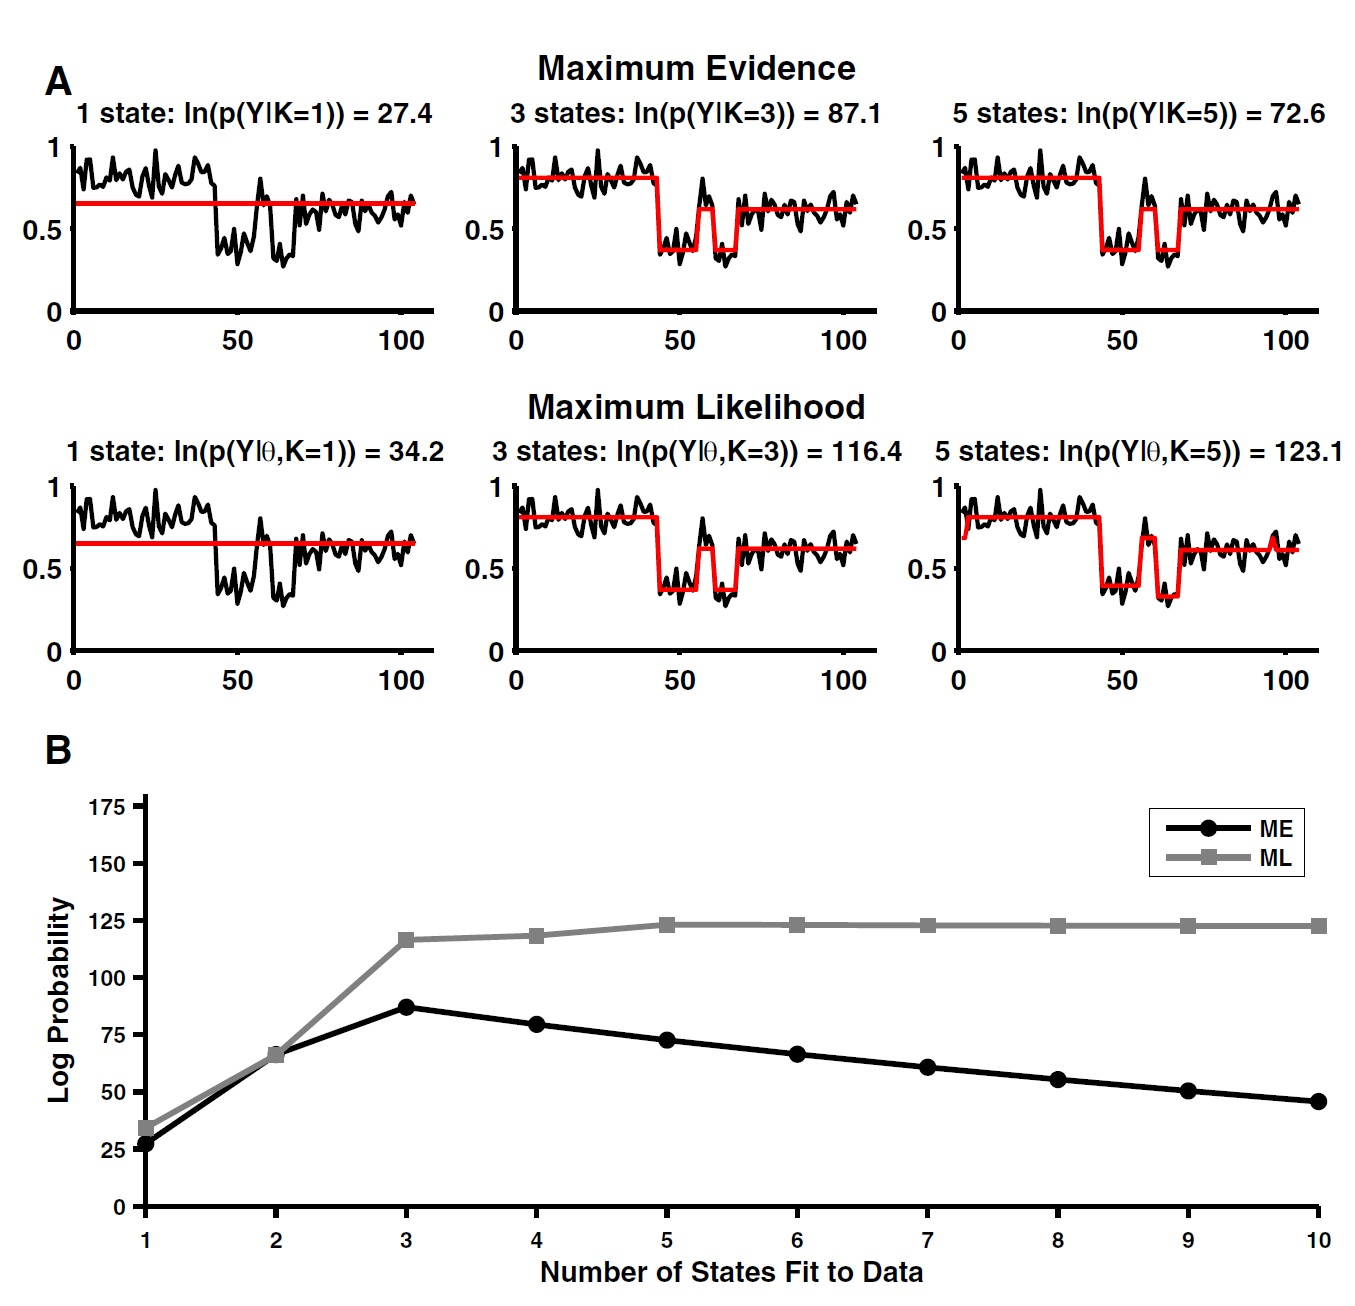
\includegraphics[height=10cm]{fig_vbms.jpg}\\
      \caption{VBEM 法的模拟结果}
      \label{fig:vbem}
    \end{figure}

    计算模拟发现,使用VBEM 改进后的隐马尔可夫模型可以识别过拟合。对于一段人工随机生成的,包含三个状态的荧光轨迹(Figure \ref{fig:vbem}a),作者比较了两种处理方法下得到的不同结果。对于欠拟合和恰好拟合情况$K=1, 3$,两种方法给出了十分类似的结果。但在$K=5$的过拟合情况下,ML 法给出了比$K=3$ 的情况下更高的概率,倾向于过拟合结果。而ME法下,$K=5$ 时的概率比$K=3$时更差,体系识别出了冗余的模型状态数。从$K=5$ 时得到的优化结果来看,被ML法认为是不同状态的两个小平台被ME 法归在了正确的类中,给出了更准确的结果。

    更准确的计算比较了不同的$K$值对这段轨迹的优化结果的影响(Figure \ref{fig:vbem}b). 当体系的状态数增大的时候,ML法给出的概率是单调增长的,而ME 法给出的结果则有一个明显的最大值。据此我们可以判断系统最可能有3个状态数,这和我们的生成这段轨迹时的参数相同。


\section{Discussion}\label{chapter:Discussion}
在本文中,我们先后介绍了处理FRET 荧光轨迹以解析微观状态信息的常规HMM方法,适用于高时间分辨率下单光子测量的H$^2$MM方法以及对参数预测和状态数预测进行了改进的VBEM 方法。常规HMM方法对于分析时间分辨率为毫秒量级,不同微观状态荧光发射峰充分分离的荧光轨迹表现较好;对于一个计算流程,常规HMM方法需要递归地优化已知荧光轨迹$y$时的隐状态数$S$,模型参数$\lambda$和隐状态链$z$。

对于常规HMM,模型假设每个时间步长探测到的光子数足够多,采集到的荧光轨迹是在不同FRET效率附近涨落的连续信号。而对于时间分辨率达到亚微秒量级的单光子探测,采集到的荧光轨迹是不同时刻的光子发射事件,状态转换呈现为光子探测事件之间的时间间隔分布而不是荧光效率的大小,此时HMM 方法不再适用。而H$^2$MM方法通过构造一个依赖于步长的状态转移矩阵,通过已知光子发射时间序列$\Delta t_n$实现了对状态链的预测。不足之处在于,目前的H$^2$MM 方法需要已知总微观状态数,这使得H$^2$MM 不能适用于仅通过荧光效率分布无法分辨不同微观状态的体系。

而在模型选择和参数优化算法中,常规HMM存在两个主要缺陷:由于常规HMM 试图在状态链未知时仍然采取最大似然估计ML法预测模型参数,HMM采用优化后验概率得到的最似然状态链$z^*$ 作为参数优化步骤中的输入状态链,这一处理方式欠缺严谨性,而且直接以最优的$z^*$代替观测$z$的做法进一步放大了模型误差。对状态数S的估计同样存在不足;基于ML方法的状态数预测将不同S 取值的先验概率视为相等,因此不能识别过拟合问题,容易使预测的$S$偏大。

VBEM算法解决了这两个问题:基于EM 算法严格化了对$p(y,\theta|K)$的处理,避免了用预测状态链近似实际状态链引入的误差。而对于状态数估计,ME方法将模型复杂度的出现权重考虑在内,使得过于复杂的模型不易出现,对$S$预测的准确度较之ML方法有明显提升。


\section{Acknowledgement}
    滕达完成了文章的第\ref{chapter:H2MM}, \ref{chapter:VBEM} 两个章节,乔卓然完成了文章的导语和第\ref{chapter:HMM}, \ref{chapter:Discussion} 章。两人共同修订并统稿了整篇文章。其中,乔卓然选定了本综述讨论的文献;他在赵新生教授实验室的工作和荧光轨迹的分析有关。


\small
\bibliographystyle{pkuplain}
\bibliography{ref}



\end{document}
